\begin{frame}{Why it is used: the constructive way}
  \begin{itemize}
    \item combat fraud or credential hijacking
          \begin{figure}
            \centering
            \begin{subfigure}{0.45\textwidth}
              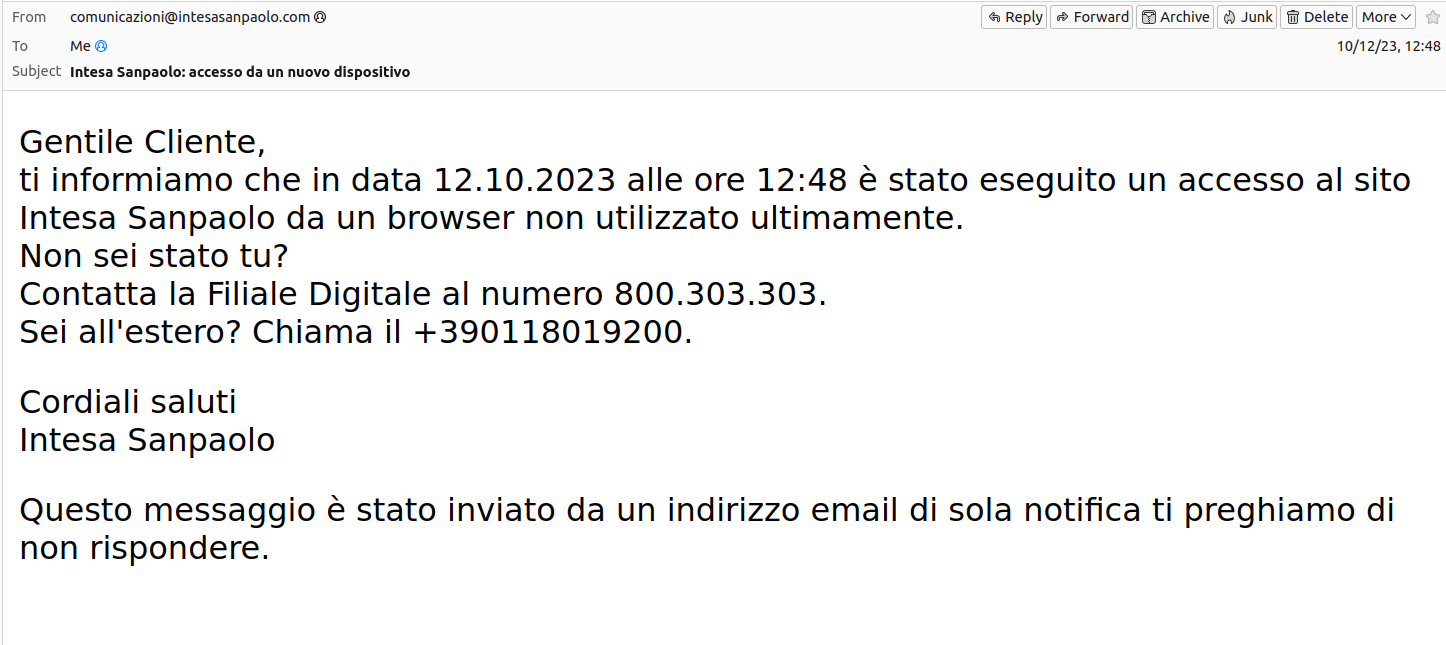
\includegraphics[width=\linewidth]{images/sanpaolo.png}
            \end{subfigure}
            \begin{subfigure}{0.45\textwidth}
              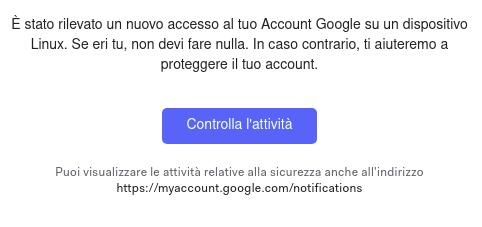
\includegraphics[width=\linewidth]{images/google.png}
            \end{subfigure}
          \end{figure}
    \item suggest updates
          \begin{figure}
            \centering
            
\includegraphics[width=0.6\linewidth]{images/update.png}
          \end{figure}
    \item bot detection
          \begin{figure}
            \centering
            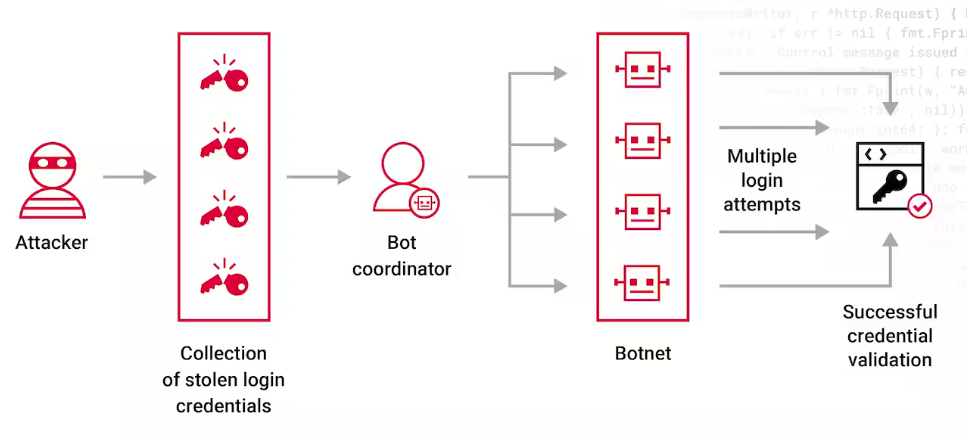
\includegraphics[width=0.6\linewidth]{images/botnet.png}
          \end{figure}
  \end{itemize}
\end{frame}

\begin{frame}{Why it is used: the questionable way}
  Track users across websites and collect information about their habits and their tastes without the users knowing about it:
  \begin{itemize}
    \item \textbf{Advertising:} data collected allows advertising businesses to create a custom profile for targeted advertising
          \begin{itemize}
            \item higher revenue for the company
            \item user satisfaction (sometimes)
          \end{itemize}
    \vspace{0.5cm}
    \item \textbf{Dynamic content and pricing:} adapt content and prices due to users habits, status and location
          \begin{figure}
            \centering
            \begin{subfigure}{0.45\textwidth}
              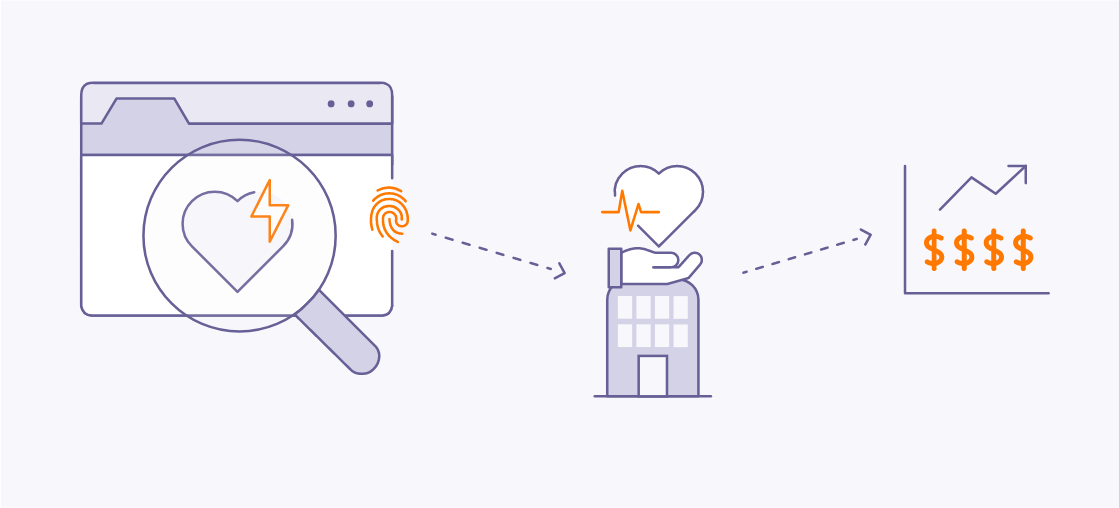
\includegraphics[width=\linewidth]{images/health.png}
            \end{subfigure}
            \begin{subfigure}{0.45\textwidth}
              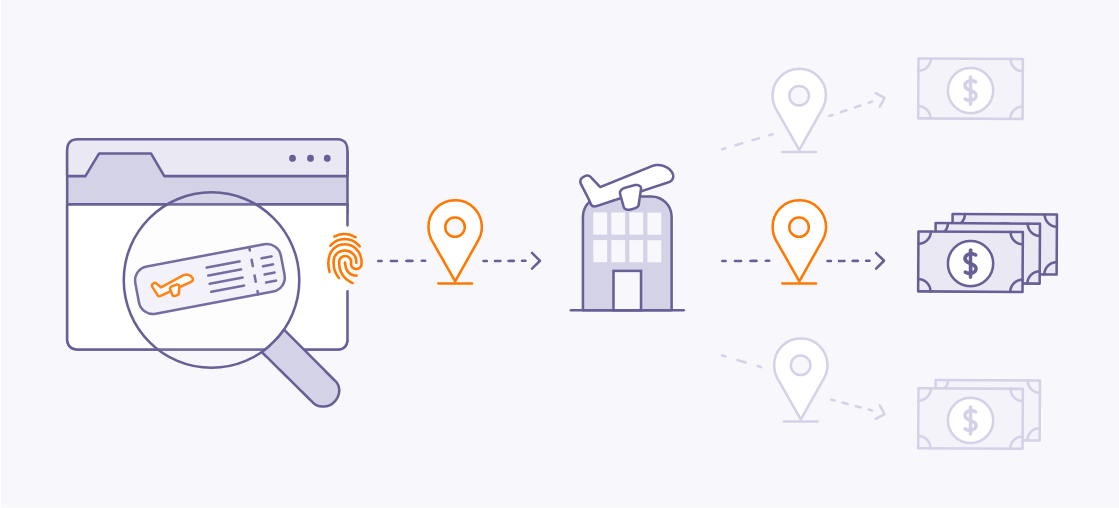
\includegraphics[width=\linewidth]{images/flight.png}
            \end{subfigure}
          \end{figure}
  \end{itemize}
\end{frame}

\begin{frame}{Why it is used: the destructive way}
  Deliver exploits that are tailored for a specific user configuration:
  \vspace{0.5cm}
  \begin{enumerate}
    \item find a website vulnerability
          \vspace{0.5cm}
    \item use this vulnerability to inject a tracking script
          \vspace{0.5cm}
    \item collect user information
          \vspace{0.5cm}
    \item define an exploit for the user
          \vspace{0.5cm}
    \item send the exploit to the user the next time he visits the website
  \end{enumerate}
\end{frame}
